%=================================================
% CHAPITRE 4 : Release 2
%=================================================

\chapter{Release 2 : Studio documentaire, production et archivage}

\section{Introduction}

La deuxième release transforme le socle technique en outil directement exploitable par les services administratifs. Les données configurées dans la première release deviennent la matière première du studio documentaire. Cette release regroupe le sprint 3, centré sur les modèles et la fusion, et le sprint 4, consacré à la génération, l'archivage et l'audit.

\section{Sprint 3 : Studio d'édition et intelligence documentaire}

\subsection{Objectif du sprint}

Le sprint 3 avait pour objectif de permettre aux administrateurs de concevoir des modèles documentaires sans intervenir dans le code. Un modèle devait pouvoir contenir un en-tête, un corps, un pied de page, des variables simples, des tableaux dynamiques, des images et des paramètres de mise en page. L'enjeu était de rapprocher l'expérience d'un traitement de texte tout en conservant une structure exploitable par le moteur de fusion.

\subsection{Backlog du sprint}

\renewcommand{\arraystretch}{1.4}

\begin{longtable}{|>{\centering\arraybackslash}p{1cm}|
                  >{\raggedright\arraybackslash}p{2.7cm}|
                  >{\raggedright\arraybackslash}p{8.2cm}|
                  >{\centering\arraybackslash}p{1.7cm}|}
\hline
\textbf{Id} & \textbf{Features} & \textbf{User stories} & \textbf{Priority} \\
\hline
\endfirsthead

\hline
\textbf{Id} & \textbf{Features} & \textbf{User stories} & \textbf{Priority} \\
\hline
\endhead

S3-01 & Familles documentaires &
En tant qu'administrateur, je veux définir les familles et leurs sources de données afin de préparer des documents adaptés à chaque besoin RH.
& Haute \\
\hline

S3-02 & Templates structurés &
En tant qu'administrateur, je veux composer un modèle avec en-tête, corps, pied de page et paramètres de page afin de respecter la forme officielle.
& Haute \\
\hline

S3-03 & Chartes graphiques &
En tant qu'administrateur, je veux réutiliser une charte par organisation afin de garder une identité visuelle homogène.
& Moyenne \\
\hline

S3-04 & Variables simples et tableaux &
En tant qu'administrateur, je veux insérer des variables et des tableaux dynamiques afin de relier le modèle aux données réelles.
& Haute \\
\hline

S3-05 & Prévisualisation avec fusion &
En tant qu'utilisateur, je veux voir le document fusionné avant génération afin de vérifier le résultat final.
& Haute \\
\hline

S3-06 & Images et pagination &
En tant qu'utilisateur, je veux que les logos, images et sauts de page restent fidèles entre l'éditeur, l'aperçu et l'impression.
& Moyenne \\
\hline

\caption{Backlog du Sprint 3}
\label{tab:backlog_sprint3}

\end{longtable}

\subsection{Analyse du sprint}

Le studio documentaire a été la partie la plus délicate du projet. Le document final doit paraître simple pour l'utilisateur, presque comme un document bureautique classique, alors qu'il dépend d'un assemblage assez dense : données SQL, modèle HTML, charte graphique, sections, variables et pagination. Pendant les tests, les problèmes les plus visibles n'étaient pas toujours les plus difficiles techniquement : un alignement d'image ou un tableau mal rendu suffit à faire perdre confiance dans tout le document. Le choix d'un éditeur riche devait donc rester compatible avec une génération contrôlée. L'application stocke les sections du modèle sous forme de HTML, mais la fusion est pilotée par des services spécialisés.

Une autre difficulté concerne les variables de type tableau. Elles ne représentent pas une valeur unique, mais une collection de lignes provenant d'une requête. Le moteur doit donc produire un tableau lisible dans le document final, conserver l'ordre des colonnes choisi et éviter de déformer la mise en page.

\subsection{Conception du sprint}

\begin{itemize}

    \item \textbf{Diagramme de classes}

    Ce diagramme présente les principales entités utilisées dans le module de génération documentaire. Il met en évidence les relations entre les templates, les familles documentaires, les chartes graphiques et les configurations nécessaires au moteur de fusion.

    \begin{figure}[H]
        \centering
        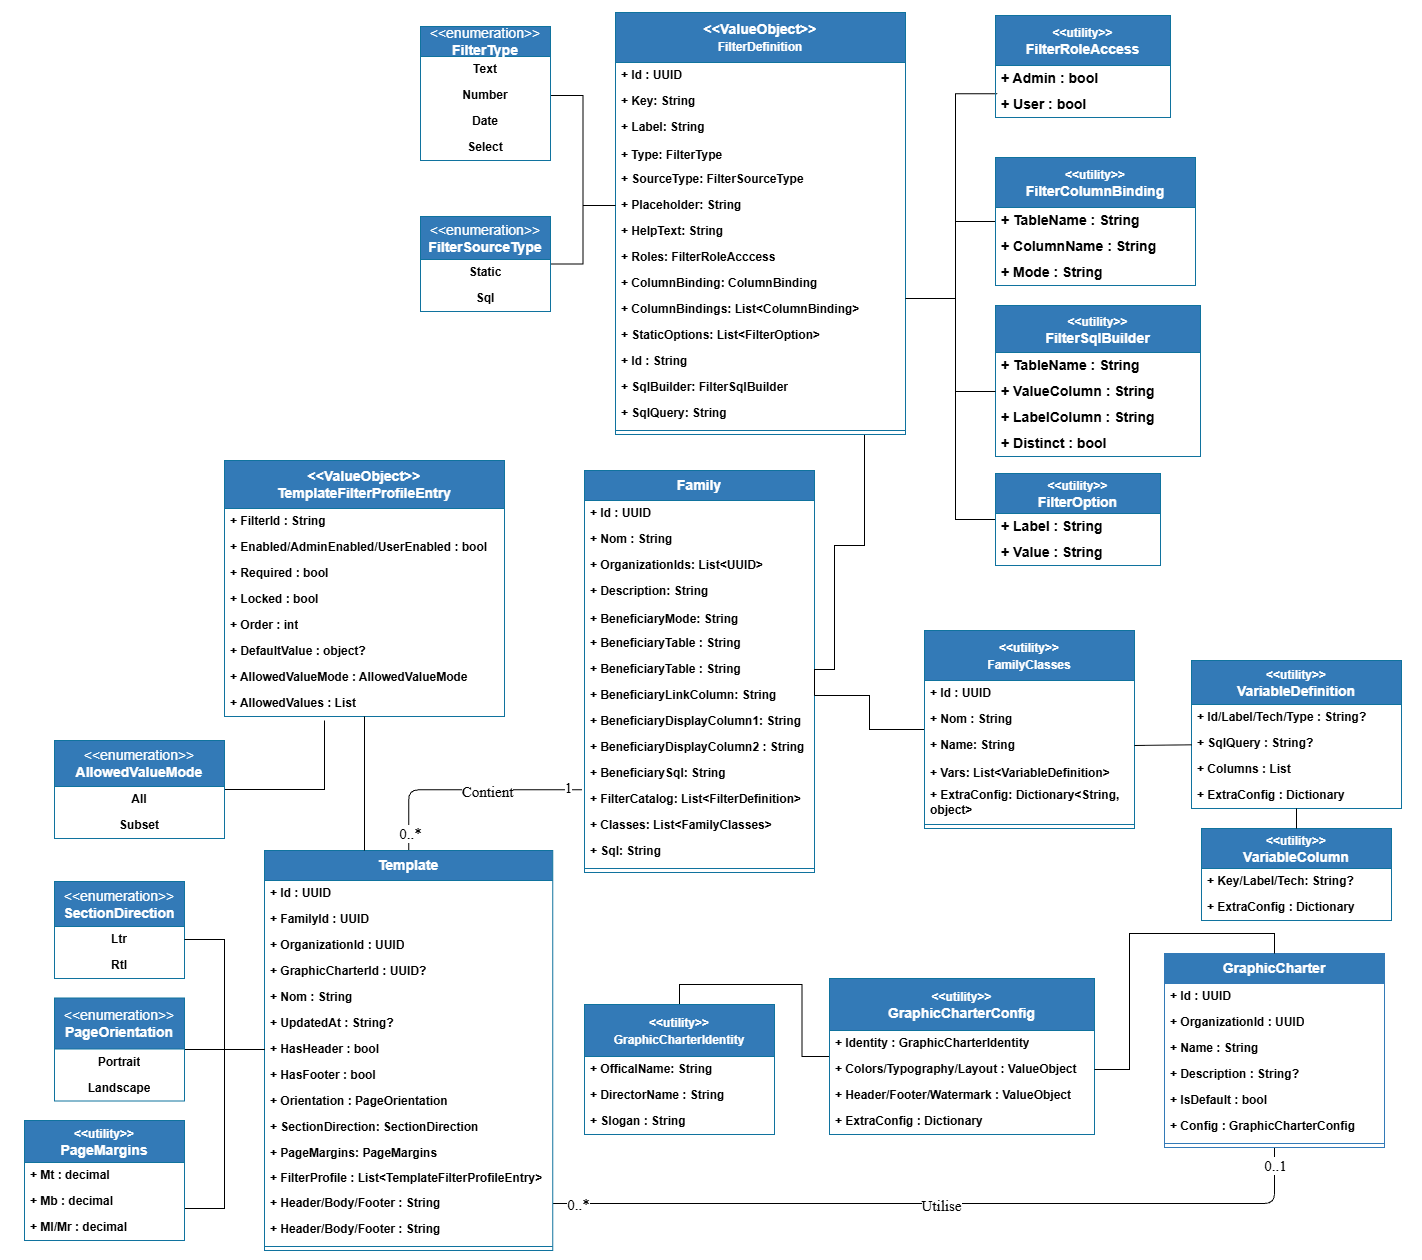
\includegraphics[width=0.95\textwidth]{images/sprint3/class-diagram.png}
        \caption{Diagramme de classes du Sprint 3}
        \label{fig:class-diagram-s3}
    \end{figure}

    \item \textbf{Diagramme de cas d'utilisation}

    Le diagramme suivant illustre les différentes actions permettant à l’administrateur de configurer les modèles documentaires, gérer les chartes graphiques et préparer les modèles destinés à la génération automatique des documents.

    \begin{figure}[H]
        \centering
        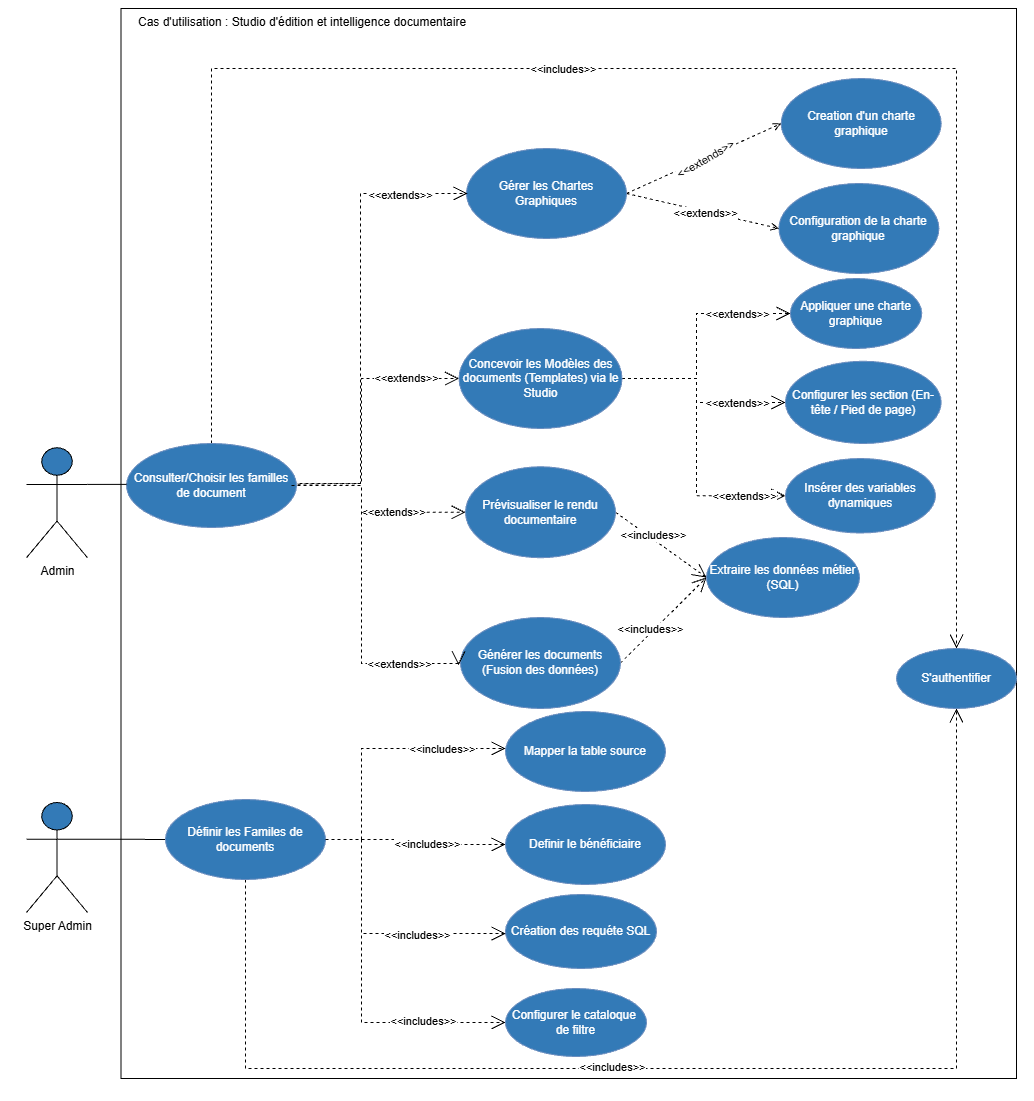
\includegraphics[width=0.9\textwidth]{images/sprint3/usecase-diagram.png}
        \caption{Diagramme de cas d'utilisation du Sprint 3}
        \label{fig:usecase-diagram-s3}
    \end{figure}

    \item \textbf{Diagramme de séquence : Enregistrement d’un template}

    Ce diagramme décrit le processus d’enregistrement d’un modèle documentaire depuis l’éditeur jusqu’au stockage dans la base de configuration. Le backend assure la persistance des différentes sections du document ainsi que des métadonnées associées.

    \begin{figure}[H]
        \centering
        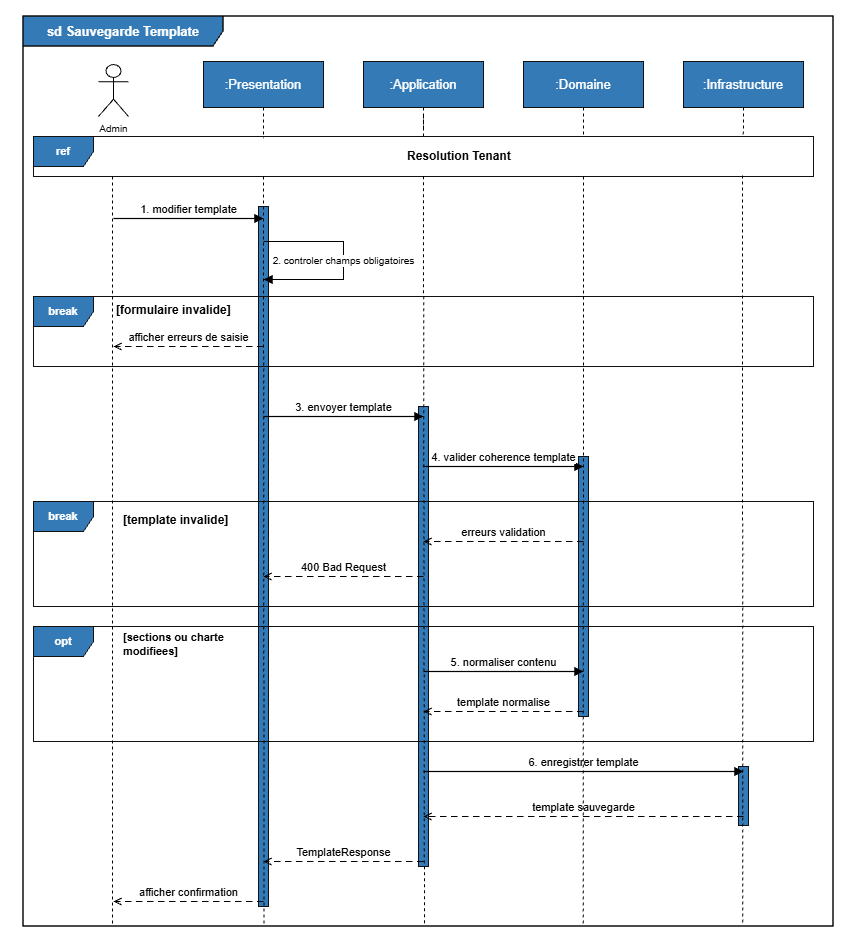
\includegraphics[width=0.95\textwidth]{images/sprint3/sequence-diagram2.png}
        \caption{Diagramme de séquence d’enregistrement d’un template}
        \label{fig:template-save-sequence-s3}
    \end{figure}

    \item \textbf{Diagramme de séquence : Prévisualisation avec fusion dynamique}

    Ce diagramme présente le fonctionnement du moteur de fusion documentaire. Le système récupère les données du bénéficiaire puis remplace dynamiquement les balises du template afin de générer une prévisualisation fidèle du document final.

    \begin{figure}[H]
        \centering
        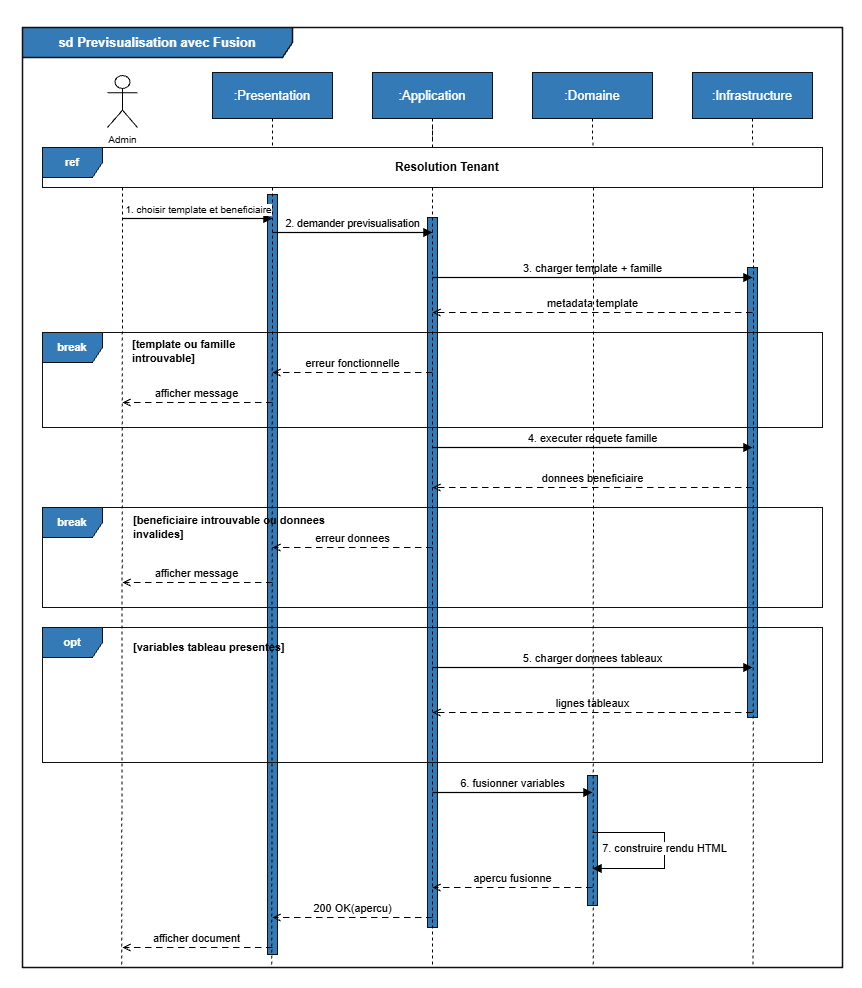
\includegraphics[width=0.95\textwidth]{images/sprint3/sequence-diagram1.png}
        \caption{Diagramme de séquence de prévisualisation avec fusion dynamique}
        \label{fig:preview-sequence-s3}
    \end{figure}

\end{itemize}

\subsection{Réalisation du sprint}

La sauvegarde des modèles s'appuie sur \texttt{TemplatesController} et \texttt{TemplateService} côté Angular. Le backend normalise les templates, puis les persiste dans la base de configuration. Les chartes graphiques sont gérées séparément afin de pouvoir appliquer une identité visuelle à plusieurs modèles.

La prévisualisation repose sur \texttt{document-data.service.ts} et \texttt{document-render.service.ts}. Le moteur récupère les données de la famille, remplace les variables, génère les tableaux, applique les styles et prépare une structure de pages. Le service de rendu prend également en charge les images afin que leur alignement reste cohérent dans l'éditeur, la prévisualisation et l'impression.

\section{Sprint 4 : Automatisation de la production et archivage RH}

\subsection{Objectif du sprint}

Le sprint 4 clôt le cycle documentaire. L'objectif était de permettre à l'utilisateur de générer un document à partir d'un bénéficiaire, de le prévisualiser, de l'imprimer ou de l'archiver, puis de retrouver cette pièce ultérieurement. Cette étape est essentielle, car elle donne une valeur administrative au document produit.

\subsection{Backlog du sprint}

\renewcommand{\arraystretch}{1.4}

\begin{longtable}{|>{\centering\arraybackslash}p{1cm}|
                  >{\raggedright\arraybackslash}p{2.7cm}|
                  >{\raggedright\arraybackslash}p{8.2cm}|
                  >{\centering\arraybackslash}p{1.7cm}|}
\hline
\textbf{Id} & \textbf{Features} & \textbf{User stories} & \textbf{Priority} \\
\hline
\endfirsthead

\hline
\textbf{Id} & \textbf{Features} & \textbf{User stories} & \textbf{Priority} \\
\hline
\endhead

S4-01 & Génération individuelle et en masse &
En tant qu'utilisateur, je veux générer un ou plusieurs documents à partir d'un modèle afin de traiter les demandes courantes plus rapidement.
& Haute \\
\hline

S4-02 & Archivage du rendu final &
En tant qu'utilisateur, je veux conserver le document généré avec ses métadonnées afin de pouvoir le retrouver plus tard.
& Haute \\
\hline

S4-03 & Filtres d'archives &
En tant qu'administrateur, je veux filtrer les archives par famille, bénéficiaire, date et générateur afin de contrôler la production documentaire.
& Haute \\
\hline

S4-04 & Visibilité par rôle &
En tant qu'utilisateur métier, je veux voir uniquement mes documents générés afin de respecter la confidentialité des productions.
& Haute \\
\hline

S4-05 & Soft-delete et audit &
En tant qu'administrateur, je veux supprimer logiquement un document afin de masquer une pièce sans perdre la trace de l'action.
& Haute \\
\hline

S4-06 & Impression et export &
En tant qu'utilisateur, je veux imprimer ou exporter un document fidèle à la prévisualisation afin de l'utiliser dans le circuit administratif.
& Moyenne \\
\hline

\caption{Backlog du Sprint 4}
\label{tab:backlog_sprint4}

\end{longtable}

\subsection{Analyse du sprint}

L'archivage a nécessité un choix important. Enregistrer uniquement un fichier final aurait simplifié la première version, mais cela aurait rendu la recherche plus pauvre et l'audit moins exploitable. SIRH-Doc conserve donc le contenu HTML final, les références au template, à la famille, au bénéficiaire et à l'utilisateur générateur. Cette approche garde une photographie du document tel qu'il a été produit, même si le modèle évolue ensuite.

Le filtrage des archives est également un point sensible. Un administrateur peut consulter les documents de son organisation, tandis qu'un utilisateur métier ne doit voir que ses propres productions. Cette règle est appliquée côté service backend, et non seulement dans l'interface, afin d'éviter une faille d'accès direct par API.

\subsection{Conception du sprint}

\begin{itemize}

    \item \textbf{Diagramme de classes}

    Ce diagramme présente les entités liées à la génération, à l’archivage et au suivi des documents produits par le système. Il met notamment en évidence la gestion des documents générés, des historiques et des traces d’audit.

    \begin{figure}[H]
        \centering
        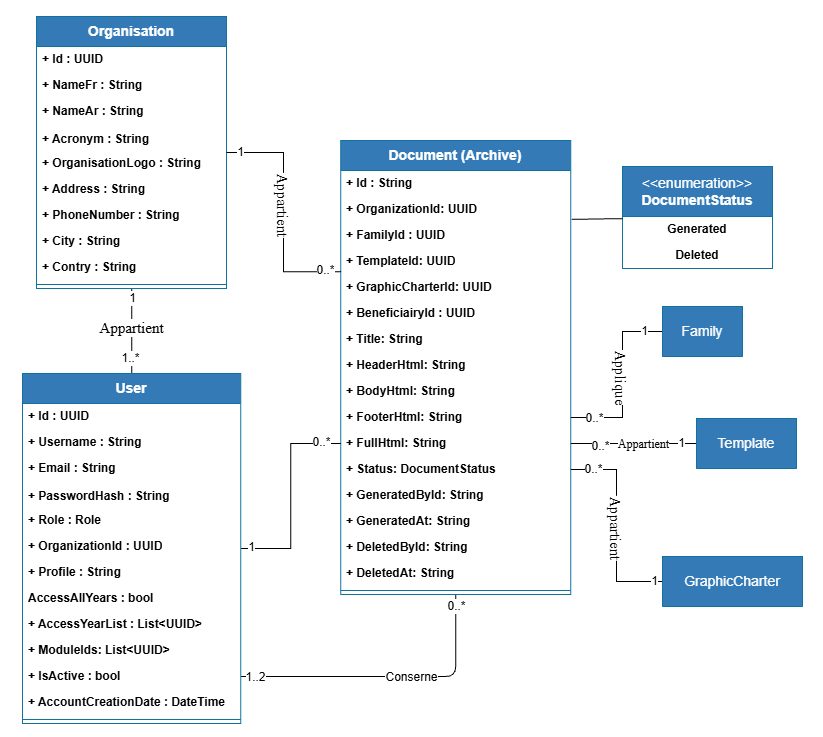
\includegraphics[width=0.95\textwidth]{images/sprint4/class-diagram.png}
        \caption{Diagramme de classes du Sprint 4}
        \label{fig:class-diagram-s4}
    \end{figure}

    \item \textbf{Diagramme de cas d'utilisation}

    Le diagramme suivant illustre les interactions des utilisateurs avec les fonctionnalités de génération, de consultation, d’impression et d’archivage des documents produits par la plateforme.

    \begin{figure}[H]
        \centering
        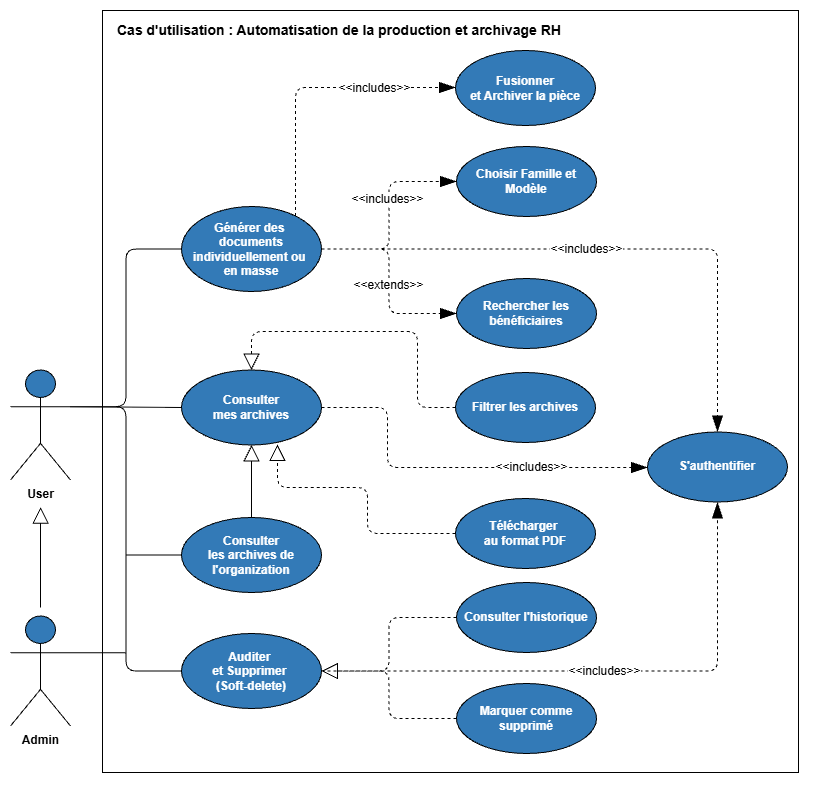
\includegraphics[width=0.9\textwidth]{images/sprint4/usecase-diagram.png}
        \caption{Diagramme de cas d'utilisation du Sprint 4}
        \label{fig:usecase-diagram-s4}
    \end{figure}

    \item \textbf{Diagramme de séquence : Génération et archivage en masse}

    Ce diagramme décrit le workflow de génération automatique de plusieurs documents. Pour chaque bénéficiaire sélectionné, le système fusionne les données, génère le document final puis l’archive afin d’assurer sa traçabilité.

    \begin{figure}[H]
        \centering
        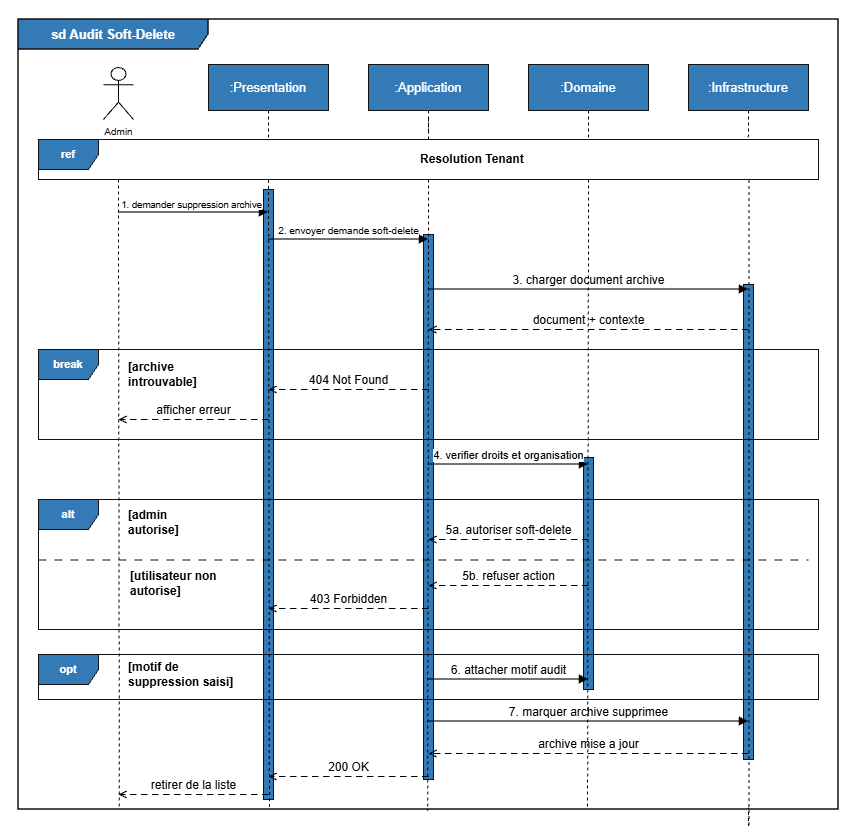
\includegraphics[width=0.95\textwidth]{images/sprint4/sequence-diagram1.png}
        \caption{Diagramme de séquence de génération et archivage en masse}
        \label{fig:bulk-generation-sequence-s4}
    \end{figure}

    \item \textbf{Diagramme de séquence : Audit et suppression logique}

    Ce diagramme présente le mécanisme de suppression logique mis en place dans le système. Lorsqu’un document est annulé, le backend conserve les informations de traçabilité afin de garantir l’intégrité de l’historique documentaire.

    \begin{figure}[H]
        \centering
        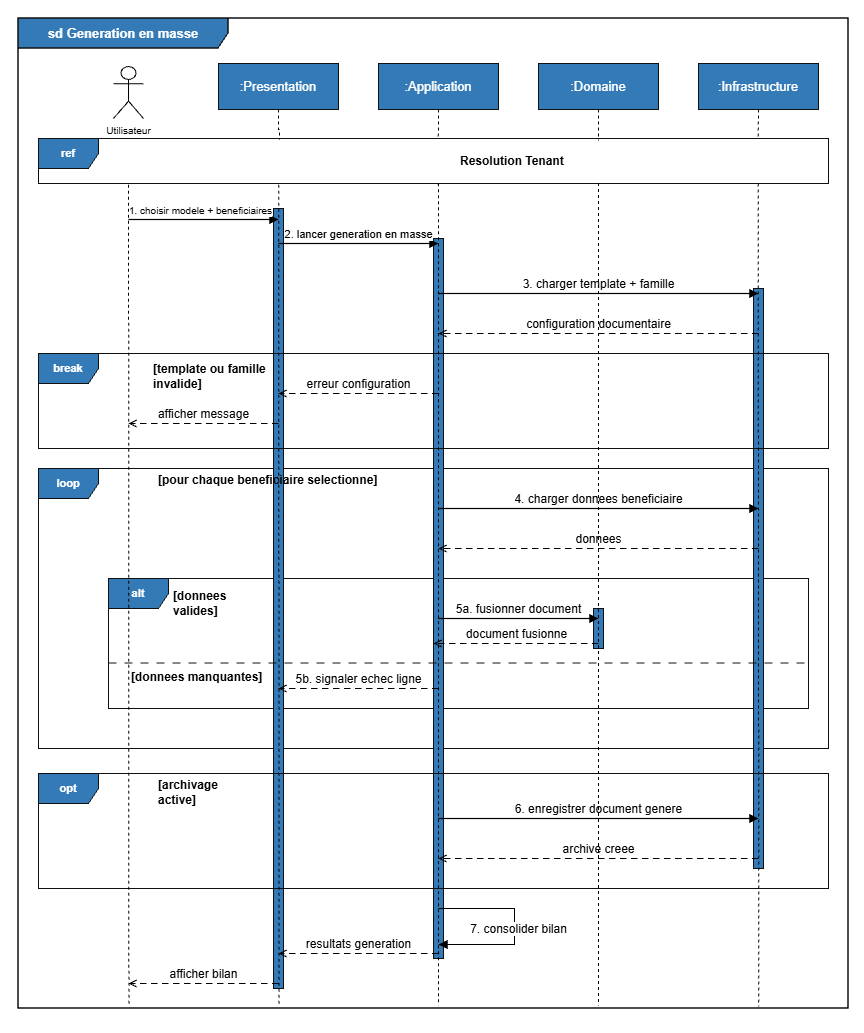
\includegraphics[width=0.95\textwidth]{images/sprint4/sequence-diagram2.png}
        \caption{Diagramme de séquence d’audit et suppression logique}
        \label{fig:audit-sequence-s4}
    \end{figure}

\end{itemize}

\subsection{Réalisation du sprint}

La production documentaire utilise les services Angular de rendu et de données, puis \texttt{DocumentService} pour l'archivage. Côté backend, les endpoints d'archives sont exposés par \texttt{EditorController}, tandis que \texttt{EditorService} applique les restrictions liées au rôle et au générateur. \texttt{EditorRepository} gère la pagination, les filtres, la création et le soft-delete des documents.

La table \texttt{document} contient les informations nécessaires à la consultation : titre, contenu HTML, identifiants de famille et de template, bénéficiaire, générateur, date de génération et statut. Pour les listes volumineuses, le backend retourne une réponse paginée afin de garder l'interface fluide.

\section{Conclusion Release 2}

La deuxième release a donné à SIRH-Doc sa dimension métier complète. Le système ne se contente plus de gérer des données ; il les transforme en documents officiels, les présente selon une charte, les imprime et les archive avec une trace exploitable. Cette release confirme l'intérêt de l'approche progressive adoptée : le studio documentaire et l'archivage reposent directement sur les choix d'isolation, de configuration et de sécurité construits dans la première release.
